% Updated October 2021 by Benjamin Herber (bherber@princeton.edu)
% 
% Document has been updated to reflect change to Docker

\documentclass[11pt, letterpaper, titlepage, oneside]{memoir}

%
% Source Code Listings
%
\usepackage{color}
\usepackage{float}
\usepackage{fontenc}
\usepackage{graphicx}
\usepackage[colorlinks=true]{hyperref}
\usepackage{listings}
\usepackage{lstautogobble}
\usepackage{parcolumns}
\usepackage{textcomp}

\definecolor{codegreen}{rgb}{0,0.6,0}
\definecolor{codegray}{rgb}{0.5,0.5,0.5}
\definecolor{codepurple}{rgb}{0.58,0,0.82}
\definecolor{backcolour}{rgb}{0.95,0.95,0.92}
\lstdefinestyle{codestyle}{
	backgroundcolor=\color{backcolour},
	commentstyle=\color{codegreen},
	keywordstyle=\color{blue}\bfseries,
	numberstyle=\tiny\color{codegray},
	stringstyle=\color{codepurple},
	numberstyle=\color{red},
	basicstyle=\footnotesize\ttfamily,
	breakatwhitespace=false,
	breaklines=true,
	captionpos=b,
	keepspaces=true,
	numbers=left,
	numbersep=5pt,
	showspaces=false,
	showstringspaces=false,
	showtabs=false,
	tabsize=2,
	upquote=true,
}

\lstnewenvironment{ruby}[1][]{
	\lstset
	{
		autogobble,
		basicstyle=\ttfamily,
		columns=fullflexible,
		breaklines=true,
		keepspaces=true,
		language=Ruby,
		frame=single,
		style=codestyle,
	}
}{}

\lstnewenvironment{bash}[1][]{
	\lstset
	{
		autogobble,
		basicstyle=\ttfamily,
		columns=fullflexible,
		breaklines=true,
		keepspaces=true,
		language=bash,
		frame=single,
		style=codestyle,
	}
}{}

\begin{document}

\mainmatter

% This chapter describes the basic building blocks
% and structures of Verilog
\chapter*{ECE 206/COS 306: \newline Software Installation Guide}
	You will be using two required programs for Verilog development
	in this class. The first,
	\href{http://iverilog.icarus.com/}{Icarus Verilog}, is a widely-used
	Verilog compiler. The scripts that we will provide to compile simulations
	of your code use Icarus Verilog. The second,
	\href{http://gtkwave.sourceforge.net/}{GTKWave}, is a simple and
	easy-to-use waveform viewer. You'll be using it in the labs to view the
	results of your simulations and debug your Verilog code. 
	In later labs, you will have the opportunity to use
	Xilinx's Vivado Design Suite to program FGPA boards using the
	lab computers in the undergraduate ELE lab and get actual working hardware!
	
	However, in a recent update to the course, we have migrated to using a \href{https://www.docker.com/resources/what-container}{Docker} image. In essence, a Docker container is a form of virtualization which is faster and smaller than a full virtual machine. The image you will be using already has iVerilog and GTKWave packaged in a Linux environment. Docker is cross-platform and provides a low bar of entry for the growing industry trend of local development.

	In addition, we strongly recommend the use of
	\href{https://code.visualstudio.com/}{Visual Studio Code} for code
	development. VSCode is a free open-source IDE that can perform syntax
	highlighting on a variety of programming languages, including Verilog. We
	recommend it because it is fast, cross-platform, and has a whole host of extensions that can be useful with Verilog, Docker, and beyond.
	All of the examples/tutorials in this course will use VSCode.
    
	There are general instructions for installation as well as some platform-specific for Windows and Unix-like (MacOS/Linux) systems. If you have difficulty getting these installations to work, contact the lab teaching assistants for help. \textbf{Please read each section carefully before you attempt them. Also, be weary of copy-pasting code from this document using your clipboard as spaces may not be preserved--all commands typically need to be executed exactly as written.}

    \section*{Installing: VSCode}
        The easy-to-install VSCode package is available at \url{https://code.visualstudio.com/}. Navigate there and download the latest version. Go through the installation and accept the license agreement. Configure the optional settings as desired. One of use may be \textit{AutoSave} which will automatically save an edited file. To enable click on \textit{File}$\rightarrow$\textit{Auto Save}. It should have a check next to it once enabled.

        \textbf{NOTE:} if you are on MacOS or Linux, please launch VSCode and type \textit{cmd/ctrl+shift+P} and type \textit{Shell Command: Install 'code' command in PATH}. Then restart any shell sessions. This will allow you to launch VSCode from the command line by simply typing \textit{code $<$file-or-dir-name$>$}. For example, \textit{code .} will open the current working directory in VSCode. This should be enabled by default on Windows.

        \subsection*{Extension: Verilog HDL}
            Now open the application (which should be in your Start Menu) and click on the last icon on the left-most bar. This should bring up the extensions toolbar. Search for \href{https://marketplace.visualstudio.com/items?itemName=mshr-h.VerilogHDL}{Verilog HDL} and install the extension named "Verilog-HDL/SystemVerilog/Bluespec SystemVerilog". This will enable syntax highlighting for Verilog in VSCode. This extension can also be configured to provide syntax checking. This will underline any syntax errors every time a file is saved. To enable syntax checking, click on the gear in the bottom-left of your VSCode window and go to settings. On the left hand side of the settings tab, click on Extensions and navigate to Verilog Configuration. Find the setting named Verilog$\rightarrow$Linting: Linter and select iverilog from the dropdown. Lastly, find the setting named Verilog$\rightarrow$Linting$\rightarrow$Iverilog: Arguments and type the text \texttt{-Wall -Wno-timescale}. Syntax checking will work once Icarus Verilog is installed and VSCode is attached to a running container.

		\subsection*{Extension: Remote - Containers}
		    The extension \href{https://marketplace.visualstudio.com/items?itemName=ms-vscode-remote.remote-containers}{Remote - Containers} allows you to attach a VSCode window to a running Docker container. As iverilog is not installed locally, this will allow you to have the aforementioned real-time linting catch errors early-on! Simply install as was done for the Verilog HDL extension.
			
		\subsection*{Optional Extension: Bracket Pair Colorizer 2}
		    Another very useful extension is \href{https://marketplace.visualstudio.com/items?itemName=CoenraadS.bracket-pair-colorizer-2}{Bracket Pair Colorizer 2}. A very common issue in Verilog is matching "begin...end" within control structures such as if statements (think like brackets '\{\}' in C or Java). This extension simply will make matching begin and end keywords distinct and matching colors: possibly helping to avoid pesky syntax errors. Simply install in the same manner as for the previous extensions.
	    
	    \subsection*{Optional Extension: Live Share}
	        The course has several large partner projects later in the semester. The extension \href{https://marketplace.visualstudio.com/items?itemName=MS-vsliveshare.vsliveshare}{Live Share} comes in very handy as it allows to to have a single, simultaneous programming session (similar to google docs) all within VSCode. Helpful documentation for the extension can be found \href{https://docs.microsoft.com/en-us/visualstudio/liveshare/use/vscode}{here}.
	        
    \section*{Installing: Docker}
        Installing Docker is fairly straightforward. Go to the \href{https://docs.docker.com/get-docker/}{Docker Website} and download the application corresponding to your operating system. Follow the instructions to install, restart your computer, and launch Docker Desktop when you log back in. For Windows users, you can safely accept the install WSL2 Backend when prompted as this is needed for Docker to run on Windows systems.

        \textbf{NOTE:} Docker Desktop must \textit{always} be running in order when you want to start a container.
    
    \section*{Installing: Command Line Tools}
        In order to provide some level of ease-of-use for this class, a few scripts have been developed. This should be the only part of installation that will be platform specific.

        \subsection*{Unix-like Systems (MacOS/Linux)}
            First, make sure Docker is running. Download the provided bash script specified for posix/unix in module on the course canvas page. Open terminal on a mac or bash on Linux and navigate to the directory containing the script \textit{ece206} (typically your downloads folder). Once there, type the commands:
            \begin{bash}
                chmod +x ./ece206
                ./ece206 init
            \end{bash}
            This will create a directory ($\sim$/ece206) in your home folder in which \textit{all} project directories must be located in order to be available within the Docker container. In order to open this directory in VSCode you can simply run the command \textit{code $\sim$/ece206}. It will also pull the latest version of the course's Docker image from the web and you may be prompted to allow the process web access. Restart your shell session, and type:
            \begin{bash}
                ece206 --help
            \end{bash}
            If you get a bunch of text describing the script in return, you may move on.

        \subsection*{Windows Systems}
            First, make sure Docker is running. Download the provided PowerShell script specified for windows in module on the course canvas page. Open PowerShell (default on systems running Windows 7 and above) and navigate to the directory containing the script \textit{ece206.ps1} (typically your downloads folder). Once there, type the commands:
            \begin{bash}
                Set-ExecutionPolicy -ExecutionPolicy RemoteSigned -Scope CurrentUser
                code ./ece206.ps1 $PROFILE
            \end{bash}
            The first command will allow any scripts made on your computer to execute, for more information see Microsoft's description \href{https://docs.microsoft.com/en-us/powershell/module/microsoft.powershell.security/set-executionpolicy?view=powershell-7.1}{here}. The last command should open two files in VSCode. Copy the contents of ece206.ps1 into the other profile document and save it. Restart PowerShell and run the following command:
            \begin{bash}
                ece206 init
            \end{bash}
            This will create a directory (\$HOME\textbackslash ece206) in your home folder in which \textit{all} project directories must be located in order to be available within the Docker container. In order to open this directory in VSCode you can simply run the command \textit{code \$HOME/ece206}. It will also pull the latest version of the course's Docker image from the web and you may be prompted to allow the process web access. Restart your shell session, and type:
            \begin{bash}
                ece206 --help
            \end{bash}
            If you get a bunch of text describing the script in return, you may move on.

    \section*{Verification}
        Time to test if everything is working! Make sure Docker is running. Then, open your shell program (Terminal/Bash/PowerShell) and type the following:
        \begin{bash}
            ece206 start
        \end{bash}
        You should now roughly see the following:

        \begin{center}
            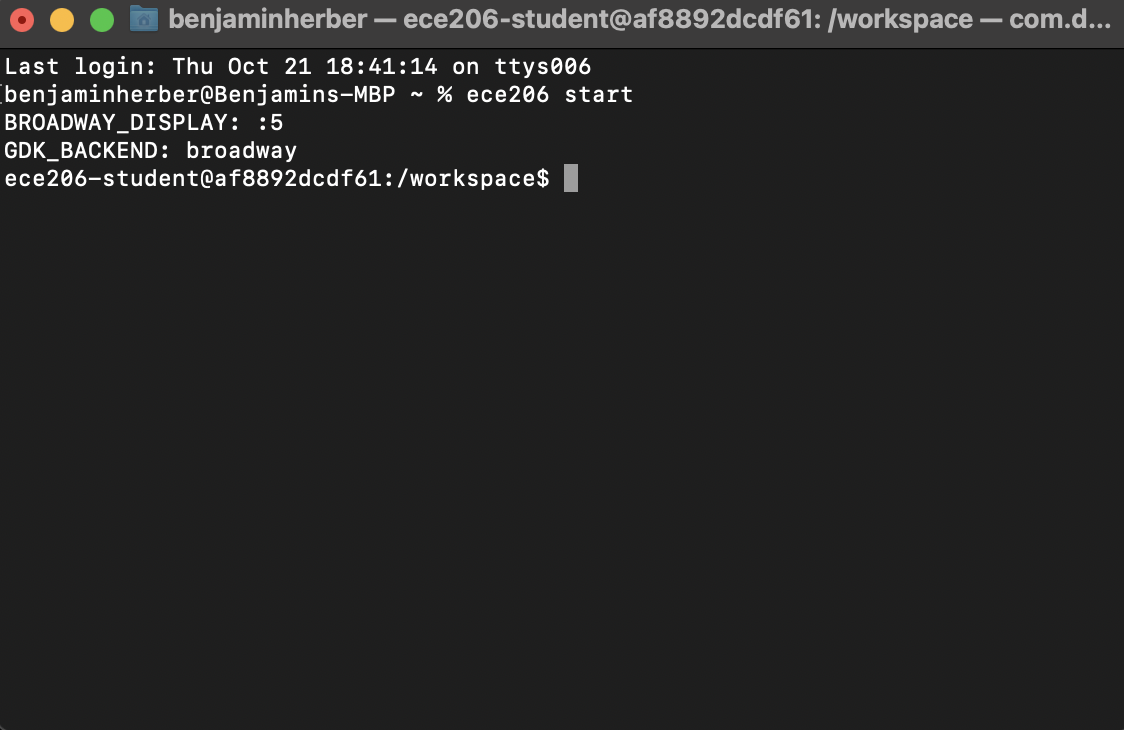
\includegraphics[width=0.6\textwidth]{./images/container_started.png}
        \end{center}
        
        Once here we can start tinkering with the software included in the image (iVerilog, Verilator, and GTKWave). You can exit the container once done by either typing \textit{exit} or pressing \textit{ctrl+D}.

        \subsection*{iVerilog}
            Test iVerilog by running:
            \begin{bash}
                iverilog -V
            \end{bash}
            You should see some legal text and other information ending with roughly the following:

            \begin{center}
                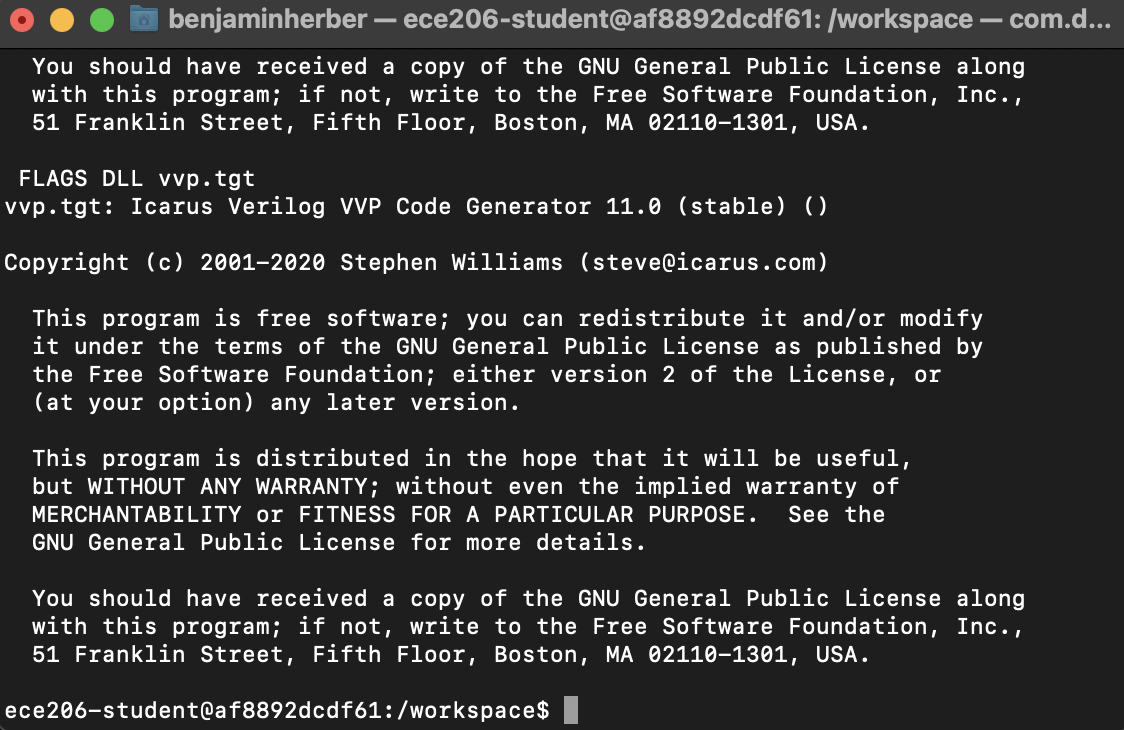
\includegraphics[width=0.8\textwidth]{./images/iverilog_confirmation.png}
            \end{center}

        \subsection*{GTKWave}
            Test GTKWave by running the following:
            \begin{bash}
                gtkwave --version
            \end{bash}
            You should see the following:

            \begin{center}
                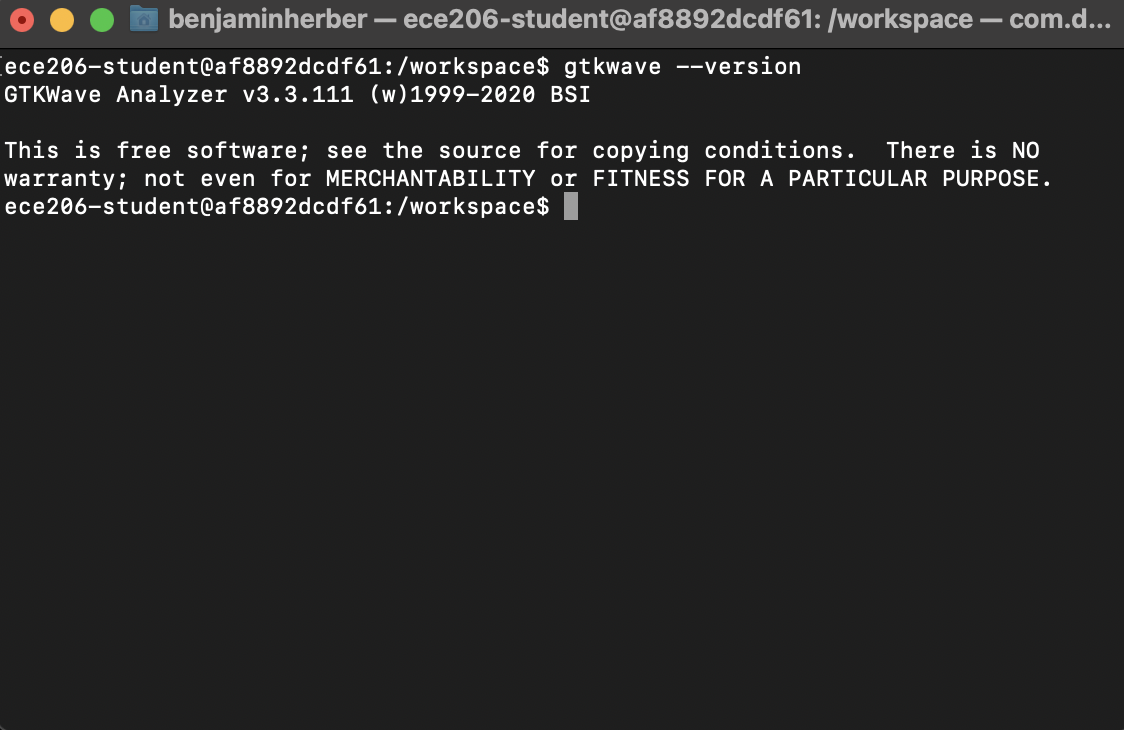
\includegraphics[width=0.8\textwidth]{./images/gtkwave_version_confirmation.png}
            \end{center}

        \subsection*{GTKWave in Browser}
            The way that we are able to access the GTKWave GUI is through a web server project called \href{https://docs.gtk.org/gtk3/broadway.html}{broadway}. Everything should be handled for you such as port-forwarding etc. To test access, simply launch GTKWave without a waveform:
            \begin{bash}
                gtkwave
            \end{bash}
            Now open your favorite browser (Chrome/Safari/Firefox/etc.) and type in the address bar:
            \begin{bash}
                localhost:8085
            \end{bash}
            
            \noindent You should see the following:
            
            \begin{center}
                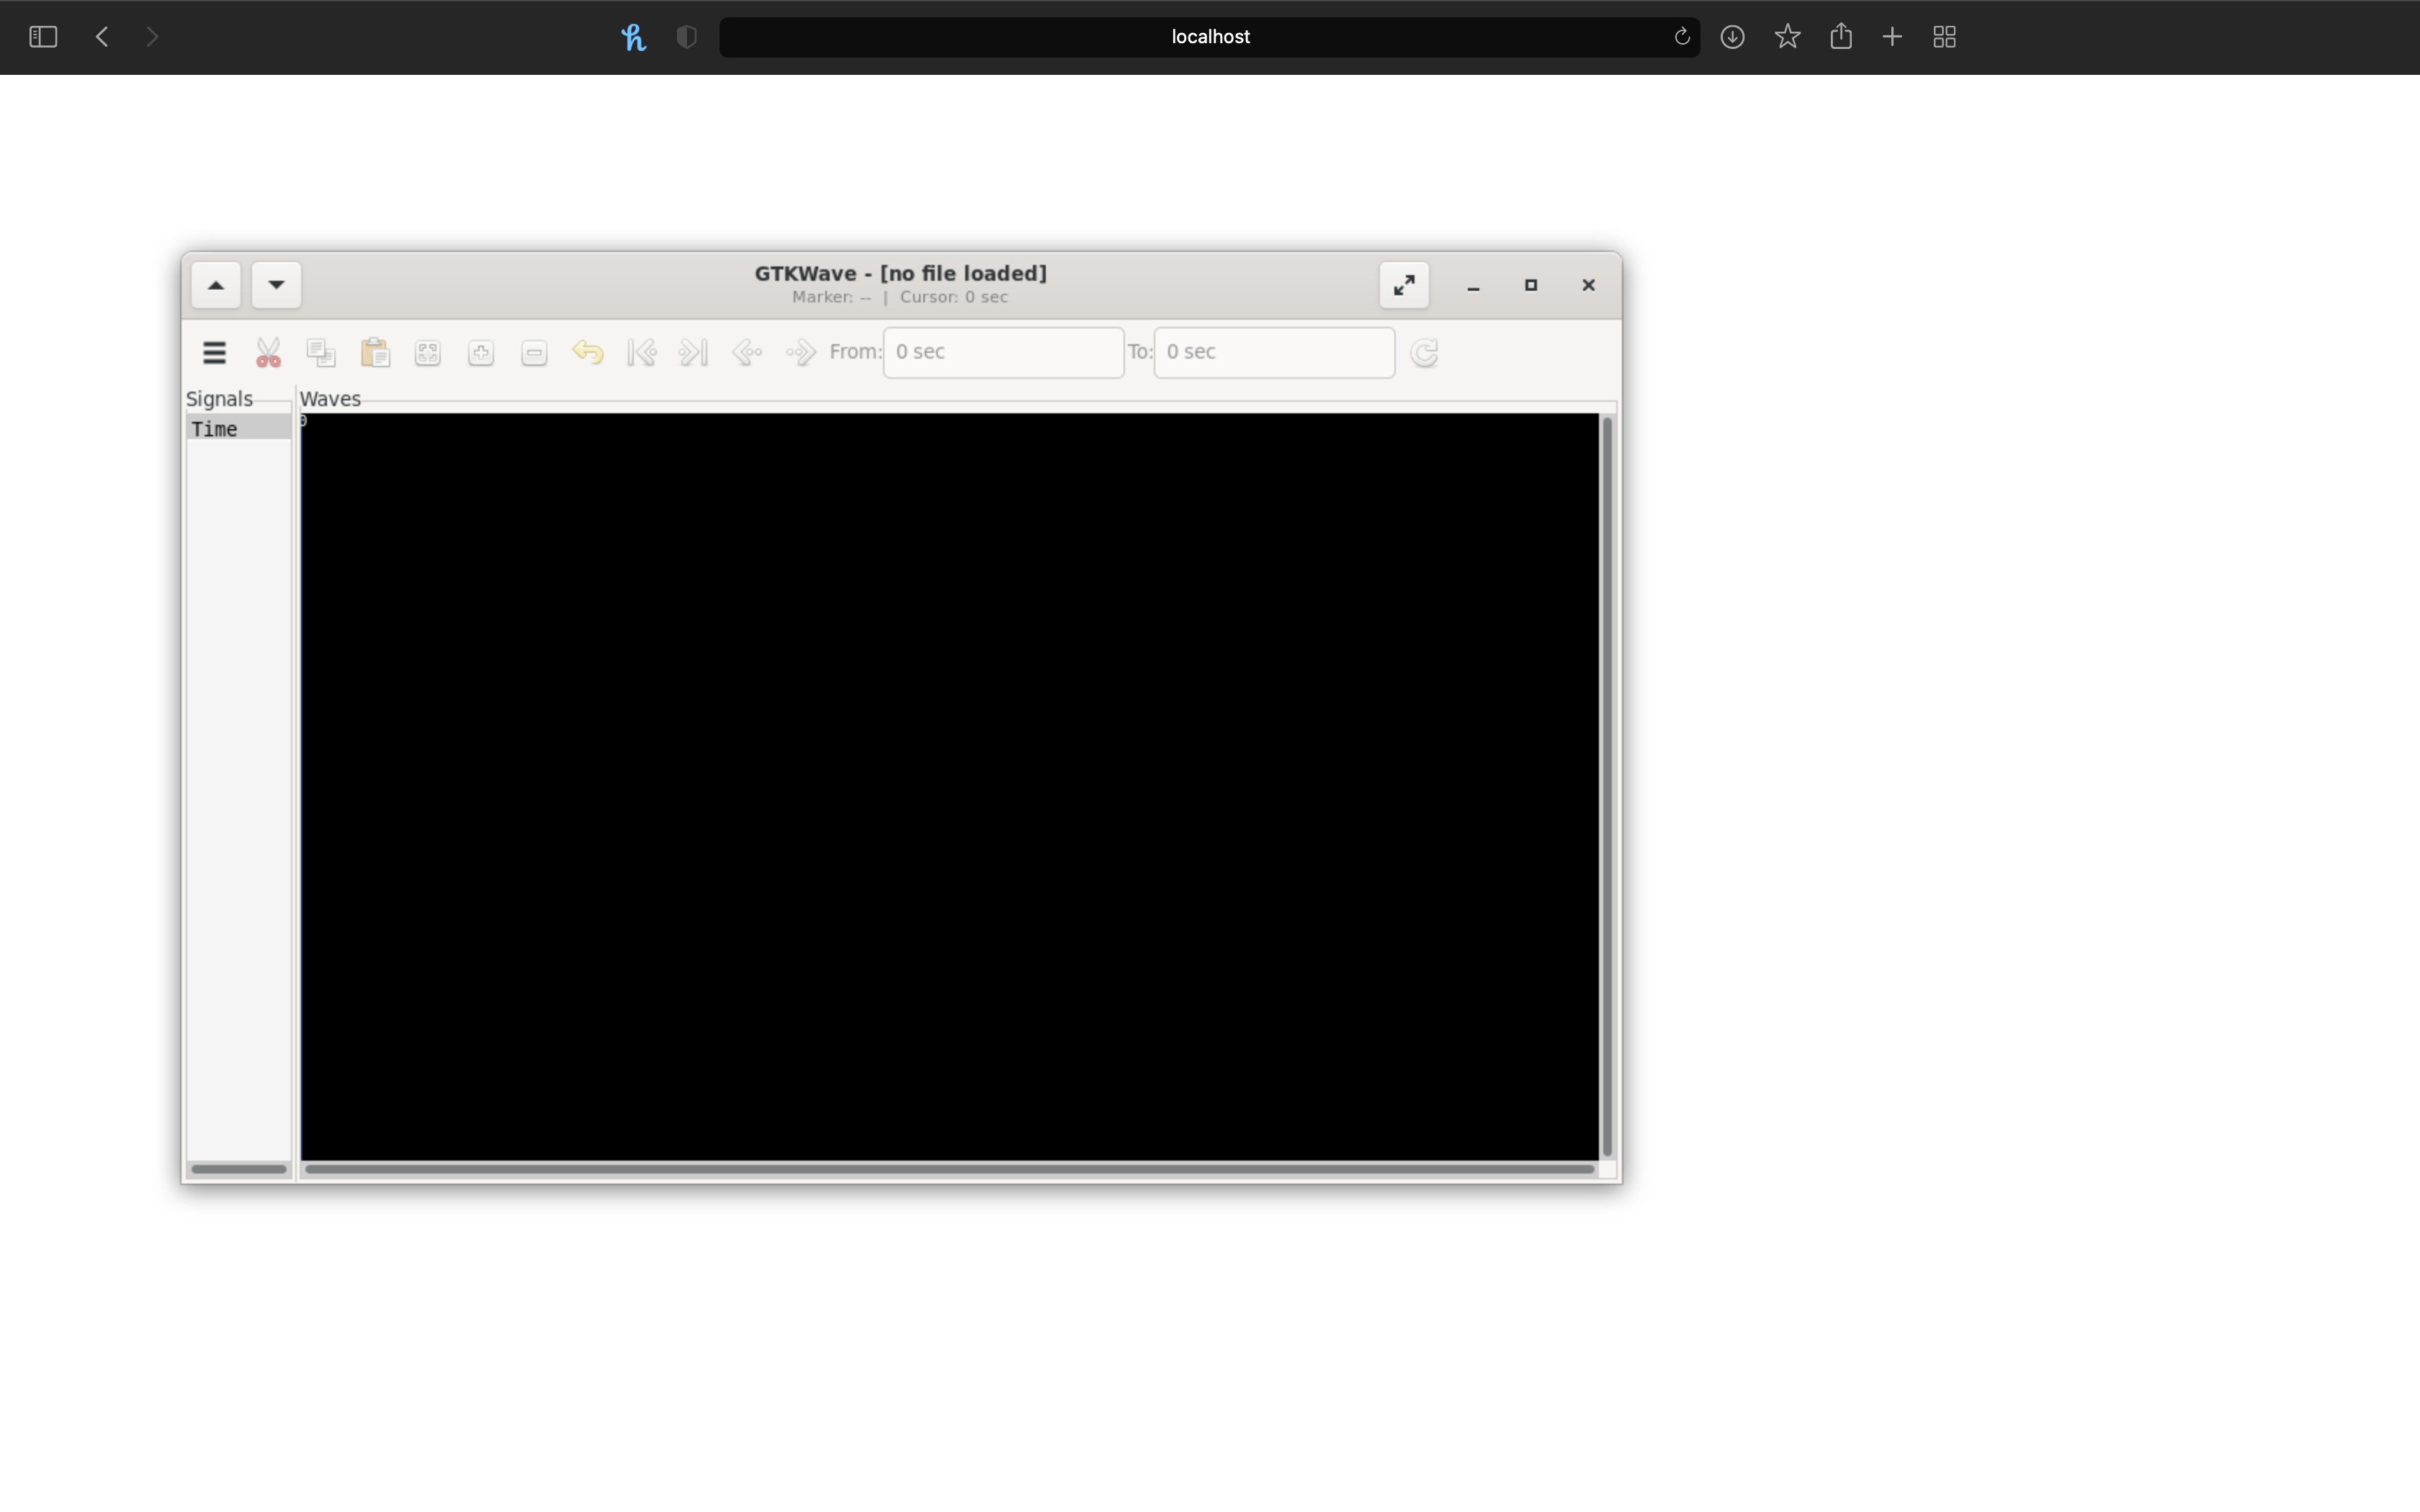
\includegraphics[width=0.9\textwidth]{./images/gtkwave_browser_confirmation.png}
            \end{center}

    \section*{How to Connect VSCode to a Container}
        In order for linting to work, VSCode needs to be able to find the iVerilog or Verilator binaries depend on which you choose to use. First, make sure that your have an active container open (i.e. you have ran and haven't closed \textit{ece206 start}). Then launch VSCode and press \textit{ctrl/cmd+shift+P}. Then type in the command palette; \textit{Remote-Containers: Attach to Running Container...} and press enter/return. You should see something like the following:
        \begin{center}
                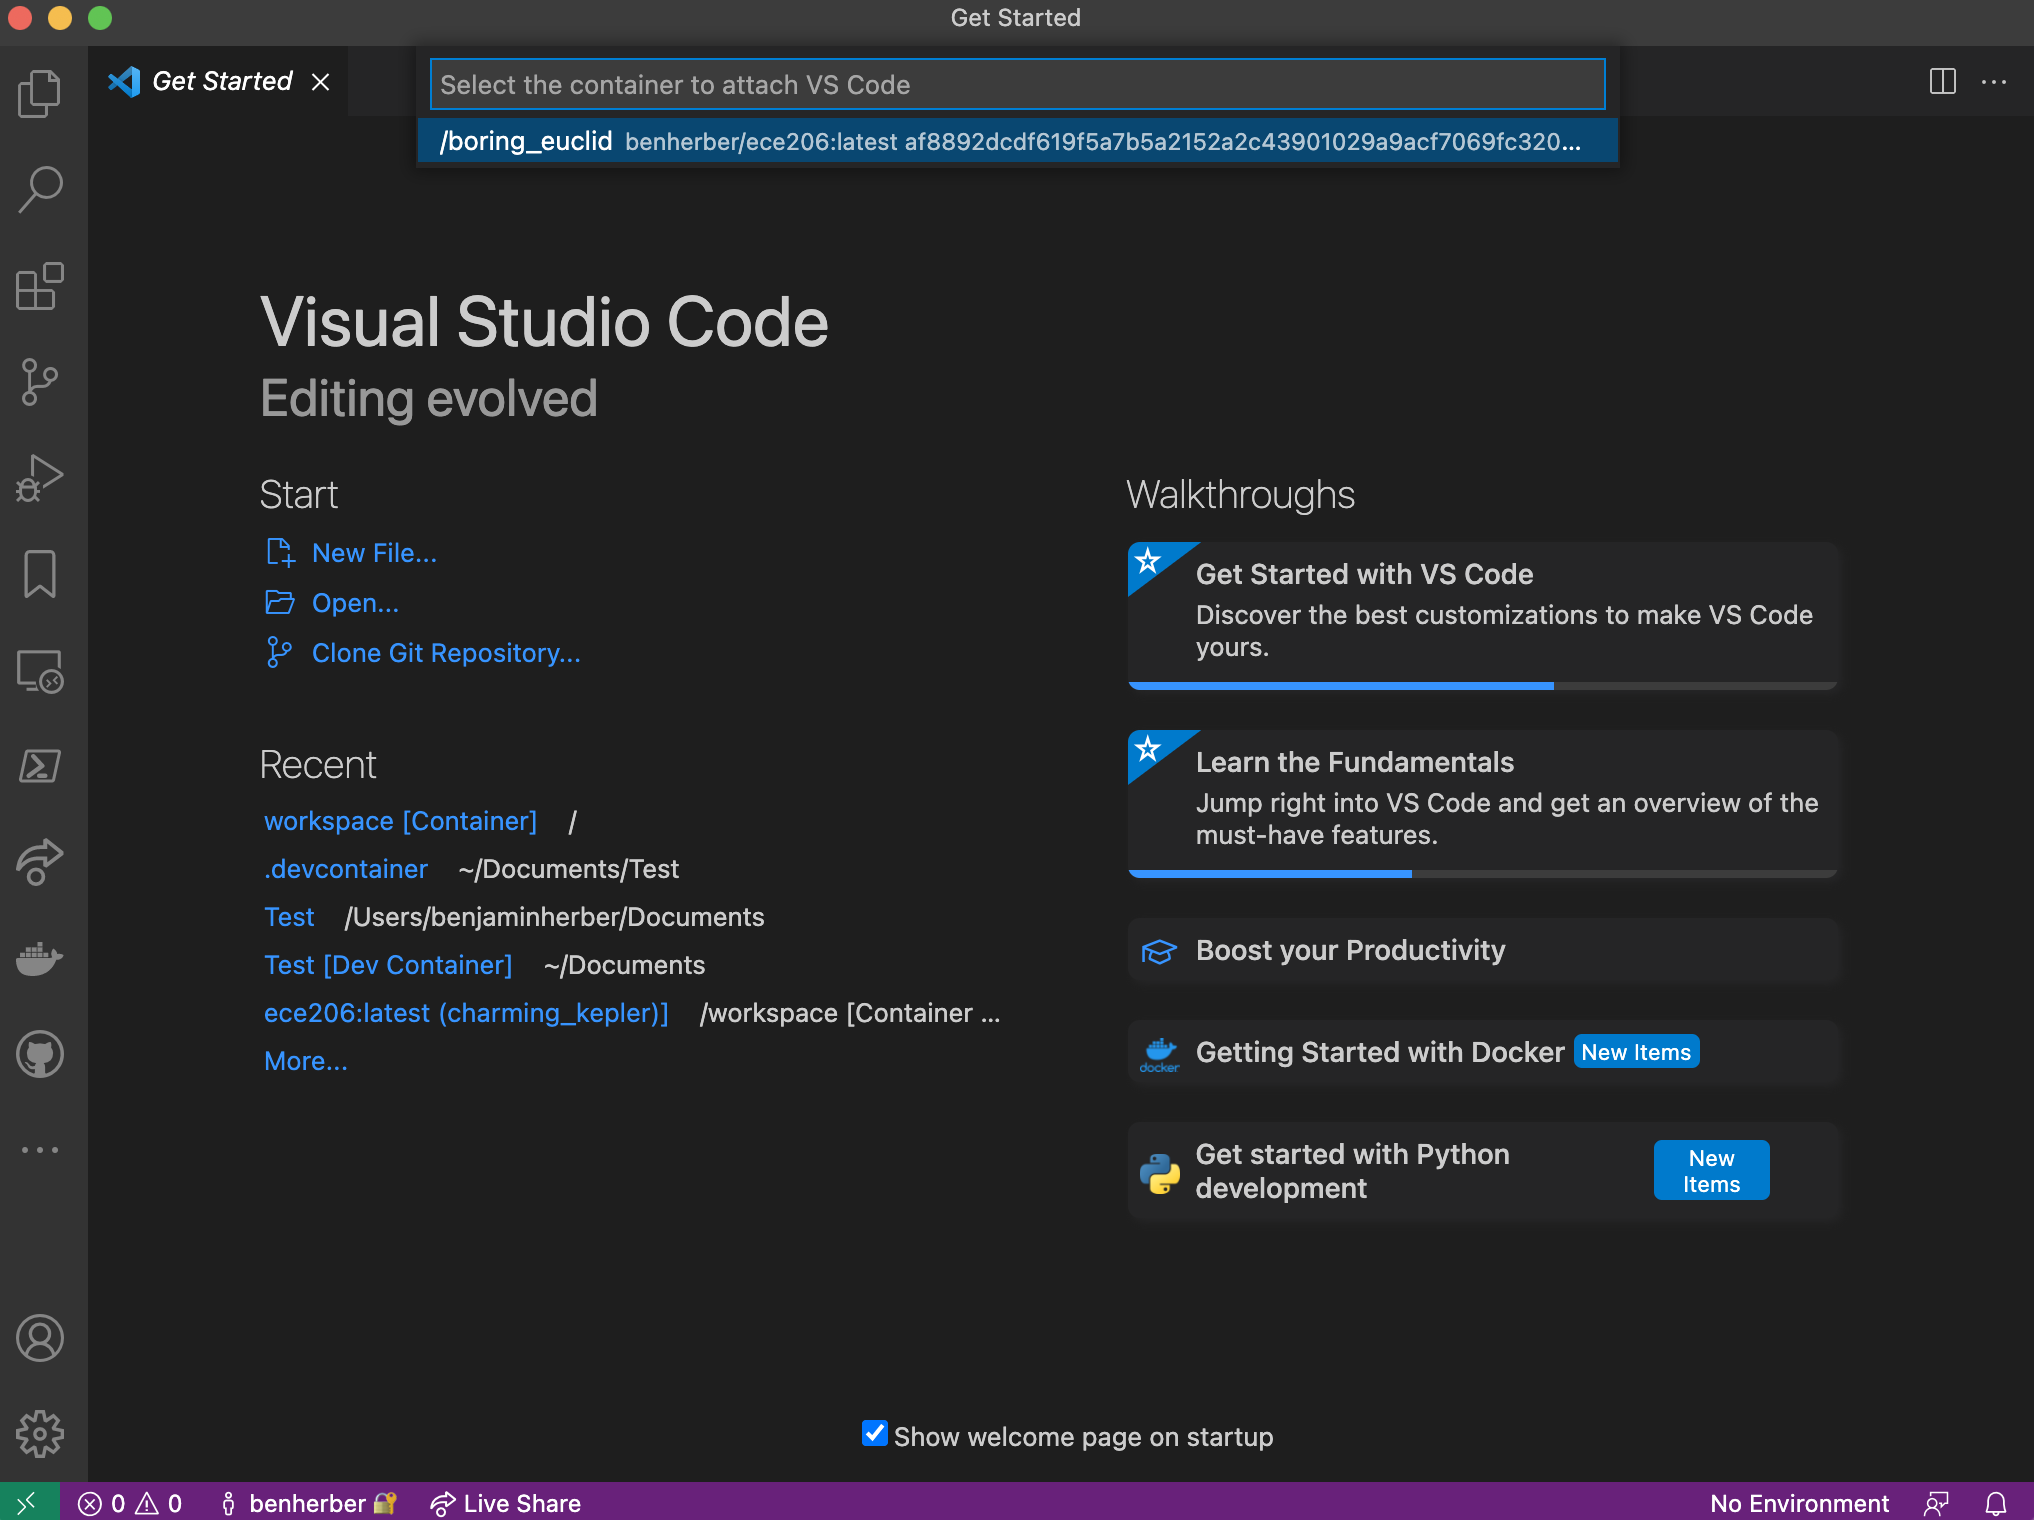
\includegraphics[width=0.65\textwidth]{./images/container_selection.png}
        \end{center}
        If you have multiple options, select the one containing \textit{benherber/ece206}. It may take a moment for VSCode to connect and install the VSCode server within the container, but once it completes, we need to navigate to the mounted directory. In order to do so, click on the File in the NavBar and press \textit{Open Folder} (you may need to go to the toolbar \textit{File}$\rightarrow$\textit{Open Folder...}). and enter \textit{/workspace} in the prompt. Then press \textit{OK}. After this, any files you have in $\sim$/ece206 or \$HOME/ece206 on MacOS/Linux or Windows respectively should appear in the file explorer on the side. Also, you'll need to enable extensions in the container. You can do this by going to the extensions tab on the toolbar and pressing the download button, selecting the preferred extensions, and pressing \textit{OK}. The relevant buttons are shown in the following:
        \begin{center}
                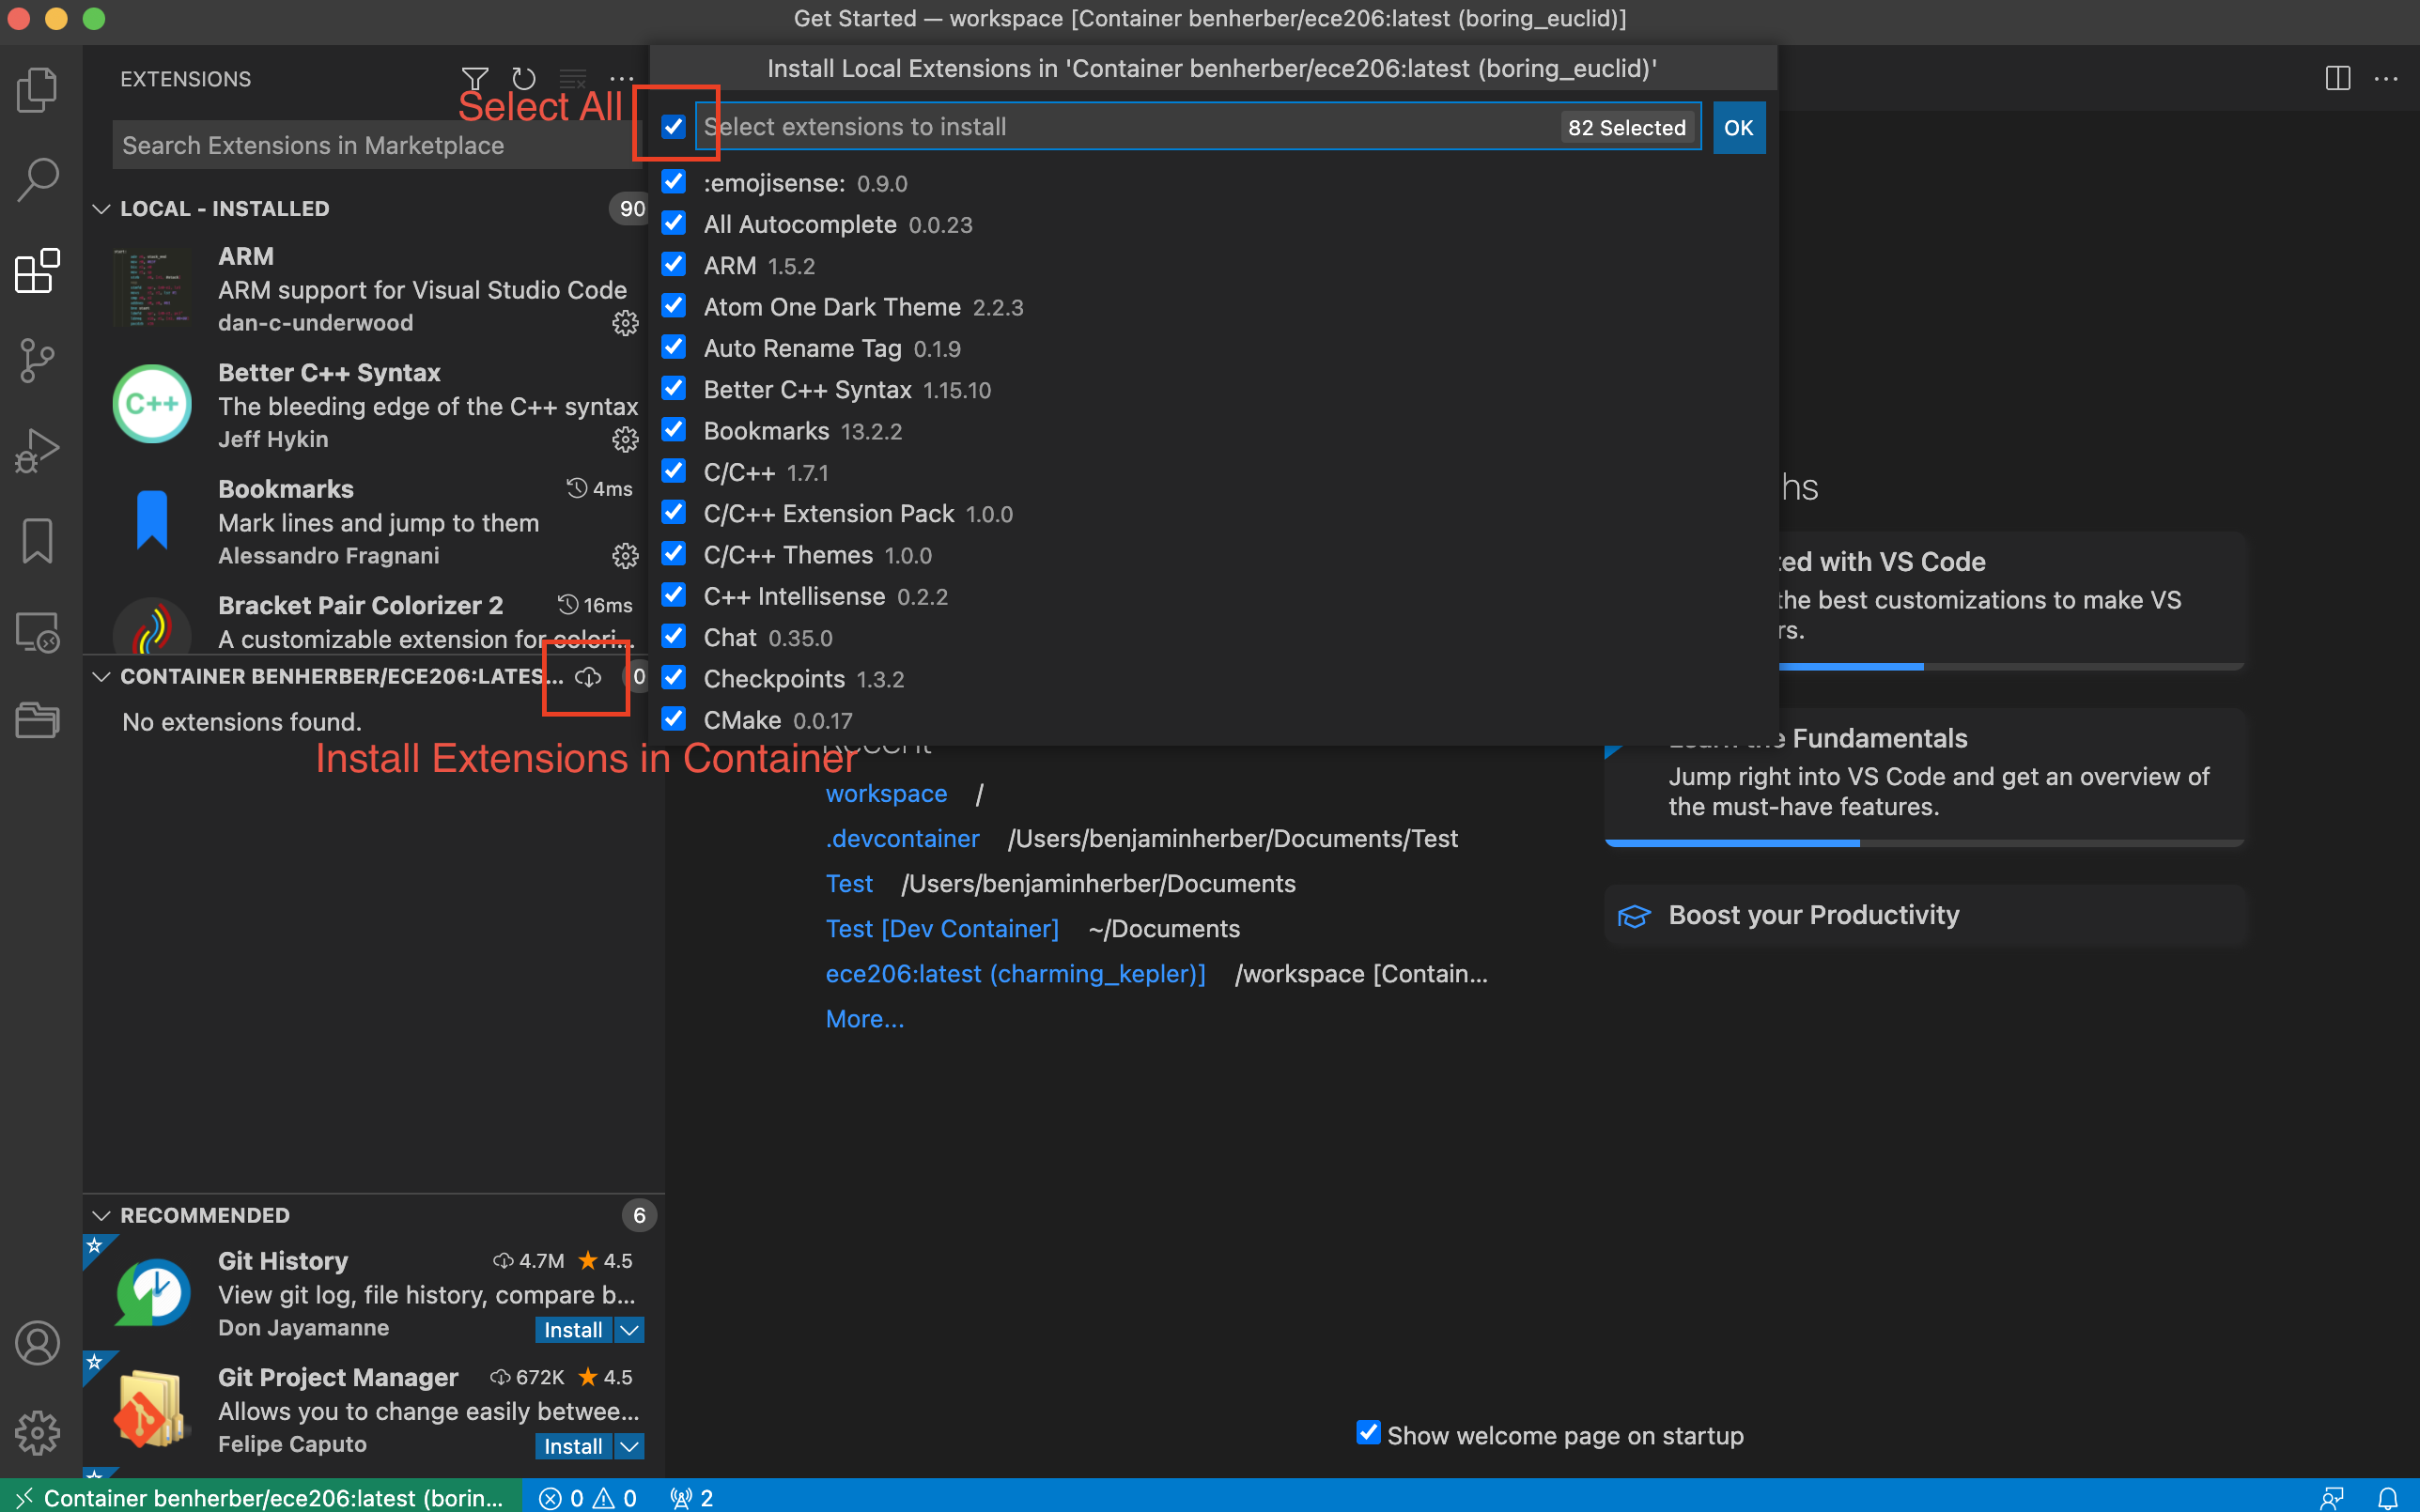
\includegraphics[width=0.75\textwidth]{./images/install_container_ext.png}
        \end{center}

    \section*{Congrats you did it!}

\end{document}
